\NewScheme{\SPOR}{SPORES}

\subsection{Message Passing through Predictive Onion Routes (PORs)}
\label{sec:message_passing}


\NewAlgorithm{\Fwd}{Forward}
\NewAlgorithm{\Send}{BuildRouteSender}
\NewAlgorithm{\Recv}{BuildRouteReceiver}
\NewAlgorithm{\ExtendRoute}{ExtendRoute}
\NewAlgorithm{\CreateOnionLayer}{CreateOnionLayer}
\NewAlgorithm{\Dec}{Dec}
\NewAlgorithm{\Store}{Store}
\NewVariable{\sk}{sk}
\NewVariable{\rdv}{rdv}
\NewVariable{\LRV}{\mathcal{L_{RV}}\xspace}
\NewVariable{\Hsend}{\mathcal{H}_{\text{send}}\begin{algorithmic}[1]}
\NewVariable{\Hrec}{\mathcal{H}_{\text{rec}}\begin{algorithmic}[1]}
\NewVariable{\Hforward}{\mathcal{H}_{\text{forward}}\begin{algorithmic}[1]}
\NewVariable{\Hbackward}{\mathcal{H}_{\text{backward}}\begin{algorithmic}[1]}
\NewVariable{\Hsendforward}{\mathcal{H}_{\text{send forward}}\begin{algorithmic}[1]}
\NewVariable{\Hsendbackward}{\mathcal{H}_{\text{send backward}}\begin{algorithmic}[1]}
\NewVariable{\Hrecforward}{\mathcal{H}_{\text{rec forward}}\begin{algorithmic}[1]}
\NewVariable{\Hrecbackward}{\mathcal{H}_{\text{rec backward}}\begin{algorithmic}[1]}


\david{each protocol should be explained individually}

The principle of onion routing à la Tor~\cite{Tor} is to put nodes relaying messages between a source and a destination.
By employing encryption layers, a relay doesn't know where it is situated on the message's path. 
It only knows who gave him the message, and where to send it to.


In contrast to Tor~\cite{Tor} that provides only one address per hop
in the route, \name provides, for each layer of the onion, several
alternative nodes for the next hop in the route depending on their
probability of being online. 
We call our modified onion routes Probabilistic Onion Routes or PORs.

Another difference from Tor, where connections are established by all nodes in the route, \name is stateless: the route's ends (the sender Alice and receiver Bob) cooperate to create the headers containing all the necessary routing information for future communication between Alice and Bob.
In that regard, two headers are required: $\Hforward$ to route packets from Alice to Bob, and $\Hbackward$ for packets from Bob to Alice.

To implement our predictive onion routing mechanism, \name is thus split in two algorithms: the route building one, and the message routing one.
Figure~\ref{fig:file-exchange} shows the process of the route creation until the first exchange of a file chunk from Alice to Bob.
Bob uses the backward route to send acknowledgments back to Alice.

\begin{figure}[t]
  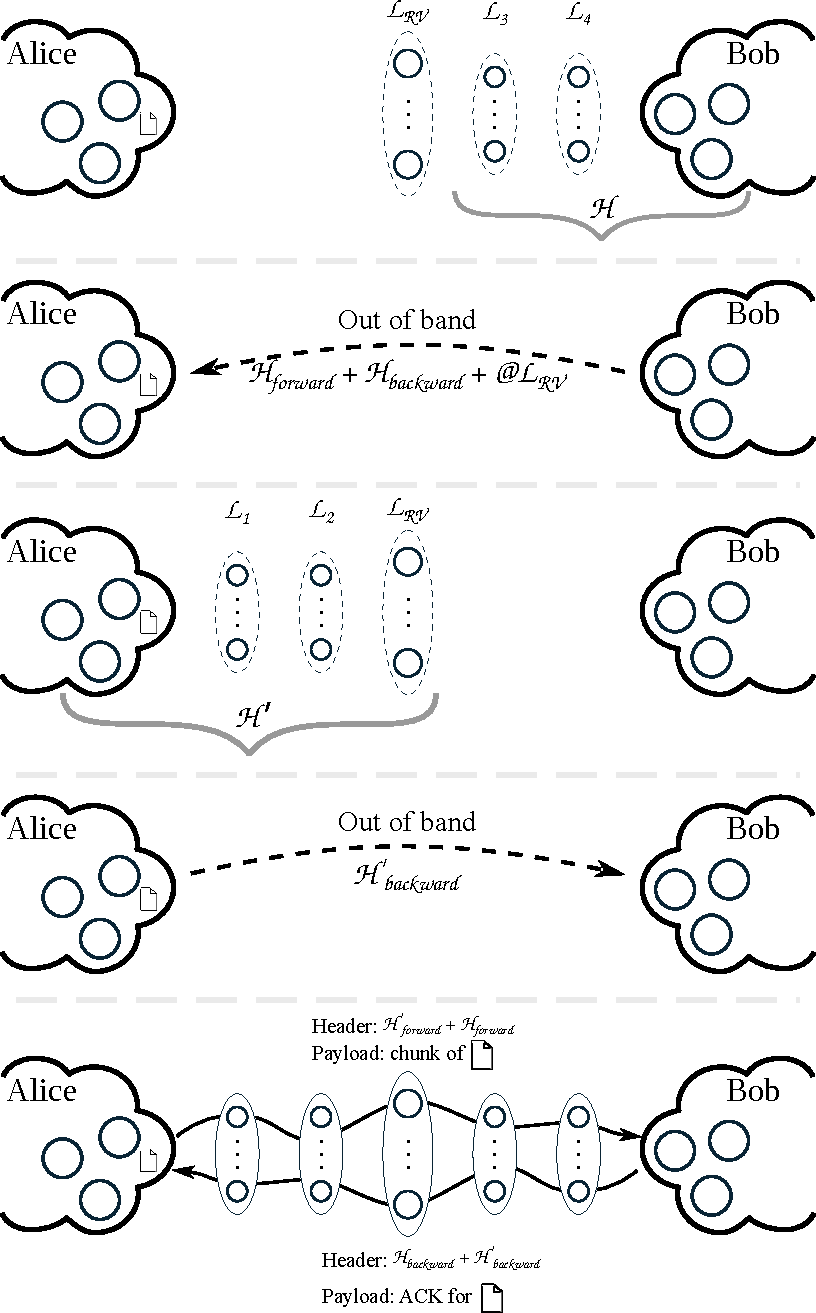
\includegraphics[width=\linewidth]{figures/file_exchange.pdf}
  \caption{\label{fig:file-exchange}A schematic of the creation and usage of PORs between Alice and Bob's e-squads.}
\end{figure}

\subsubsection{Building routes} 
\label{ssub:building_routes}



When Alice wants to send a file to Bob, they first have to call the route building algorithm, and to exchange relevant information out of band (e.g. using mail, or their phones' bluetooth connection).
They create a route of $L$ layers, a configuration parameter that must be odd. We introduce $l=(L-1)/2$.
Bob (the receiver) initiates the route creation. 
He randomly chooses nodes to constitute a rendez-vous layer \LRV, and nodes to constitute $l$ layers from \LRV to his \squad. 
We come back on layer creation below.
He crafts a layered encrypted header (more details below) to \LRV (excluded) to his squad (included), that we will call \Hrecforward.
He also crafts his part of the header for the backward route, \Hrecbackward: it contains the route from Bob's \squad (excluded) to \LRV (included).

Bob sends \Hrecforward and the descriptors of the \LRV nodes to Alice.
Alice still has her part of the route to create: like Bob, she randomly picks nodes to constitutes $l$ layers from her \squad to \LRV.

\paragraph*{Layer creation}

\paragraph*{Header preparation}

\begin{figure}[t]
  %\framebox{\begin{minipage}{0.96\linewidth}
  \begin{algorithmic}[1]
    % \Require{%
    %   $D$ is the set of alternative recipient devices.
    % }
    \Function{\Recv}{$D$}
      \State $H_\rdv\gets \ExtendRoute[D\concat \top, L, \theta]$
      \State \Return $H_\rdv$
        \Comment{Give to sender out-of-bound.}
    \EndFunction
  \end{algorithmic}
  %\end{minipage}}

  \vspace{0.3em}
  %\framebox{\begin{minipage}{0.96\linewidth}
  \begin{algorithmic}[1]
    % \Require{%
    %   $m$ is the message to be sent,
    %   $H_\rdv$ is the onion-route given by the recipient.
    % }
    \Function{\Send}{$H_\rdv, m$}
      \State $H\gets \ExtendRoute[H_\rdv, L, \theta]$
      \State $D\concat C_H\gets H_\rdv$
      \For{$d\in D$}
        \Comment{Uniformly randomly chosen}
        \If{$d\method \Fwd[C_H, m] \neq \bot$}
          \State \Return $\top$
        \EndIf
      \EndFor
      \State \Return $\bot$
    \EndFunction
  \end{algorithmic}
  %\end{minipage}}

  \vspace{0.3em}
  %\framebox{\begin{minipage}{0.96\linewidth}
  \begin{algorithmic}[1]
    % \Require{%
    %   $H$ is a header of the form \(D\concat H'\) or \(D\concat \top\), where 
    %   \(D\) is a set of device addresses.
    %   $\pk_D$ is the public key of device set $D$.
    %   $L$ is the length of the route,
    %   $\theta$ is the threshold of probability of failure.%
    % }
    \Function{\ExtendRoute}{$H, L, \theta$}
      \If{$L\leq 0$}
        \State \Return $H$
      \EndIf
      \State $D\gets \CreateOnionLayer[\theta]$
      \State $H\gets D\concat \DeBEenc[\mpk, D, H]$
      \State \Return $\ExtendRoute[H, L-1, \theta]$
    \EndFunction
  \vspace{0.3em}
    \Function{\CreateOnionLayer}{$\theta$}
      \State $(d, \pk_d, p_d)\gets \GetRandomPeer$
      \State $D\gets \{(d, \pk_d, p_d)\}$
      \While{$\prod_{d\in D} p_d > \theta$}
        \State $(d, \pk_d, p_d)\gets \GetRandomPeer$
        \State $D\gets D\cup \{(d, \pk_d, p_d)\}$
      \EndWhile
      \State \Return $D$
    \EndFunction
  \end{algorithmic}
  %\end{minipage}}
  \caption{\label{fig:route building algo}The route building algorithm}
\end{figure}

\subsubsection{Routing messages}
\label{ssub:routing_messages}


\begin{figure}[t]
  %\framebox{\begin{minipage}{0.96\linewidth}
  \begin{algorithmic}[1]
    %\Require{$\pk, \sk$ is the public--private key-pair of the node.}
    \Function{\SPOR[\Fwd]}{$C_H, m$}
      \State $H\gets \DeBEdec[\mpk, \sk, C_H]$
      \If{$H = \bot$}
        \State \Return $\bot$
      \EndIf
      \State $\{d_i\}\concat C_H'\gets H$
      \If{$C_H' = \top$}
        \State \Return $\Store[m]$
      \EndIf
      \For{$d\in \{d_i\}$}
        \Comment{Uniformly randomly chosen}
        \If{$d\method \Fwd[C_H', m] \neq \bot$}
          \State \Return $\top$
        \EndIf
      \EndFor
      \State \Return $\bot$
    \EndFunction
  \end{algorithmic}

  \begin{algorithmic}[1]
    \Function{\Store}{$m$}
      \State $m\gets \DeBEdec[\mpk, \sk, c_m]$
      \If{$m = \bot$}
        \State \Return $\bot$
      \EndIf
      \State Store $m$ to disk.
      \State \Return $\top$
    \EndFunction
  \end{algorithmic}
  %\end{minipage}}
  \caption{\label{SPORFwd}%
    The \(\SPOR[\Fwd]\) algorithm forwards \(m\) down the route \(H\), obtained 
    by decrypting \(C_H\) with the node's associated private key.
    The special value \(H = \top\) indicated the end of the route, thus \(c_m\) 
    is intended for the local node and \(c_m\) is instead sent to disk using 
    \(\Store\) (\cref{SPORRecv}).%
  }
\end{figure}


For instance, if Alice wants to send a message \(m\) to Bob, they are both going to perform a part of the building algorithm.
Bob uses the \(\SPOR[\Recv]\) function (See \cref{SPORRecv}) to create a probabilistic onion route $\mathcal{H_B}$ from
 a rendez-vous (RV) layer $\mathcal{L_{RV}}$ to its own devices from its \squad---all the hops on the route are 
chosen by Bob uniformly at random from the Global Overlay.
 \(\SPOR[\Recv]\)
returns $\mathcal{H_B}$ and  that Bob gives to Alice using an
out-of-band channel, \eg using one device of its \squad.
PORs have \(L\) layers, and for each layer the number of
alternatives nodes depends of a failure threshold \(\theta\). 
As long as \(\theta\) is not exceeded, alternatives nodes are added in
\(H_\rdv\) as depicted in \cref{ExtendRoute}. Thus the probability of
failure for the extension is \(1 - (1 - \theta)^L\).

Once Alice get the \(H_\rdv\), Alice uses \(\SPOR[\Send]\) at some
later time to send the message to Bob using any of her devices from
its \squad (See \cref{SPORSend}). First, \(\SPOR[\Send]\) extends the route
\(H_\rdv\) with some hops of Alice's choosing (uniformly randomly
chosen). Second, \(\SPOR[\Send]\) extracts from the onion the first
layer, which contained the overall
possible rendez-vous points $D$ previously selected by the recipient (i.e. Bob).
One device from $D$ is randomly chosen, and the \(\SPOR[\Fwd]\)
sub-function is called as long as the message forwarding to one node of
the next layer is not successful (See \cref{SPORFwd}). Along the path, each node decrypts
in sequence the different layer with the current node’s private key. 
The end of the route is reached when special value \(H_\rdv = \top\) is
encountered. Consequently the ciphered message \(c_m\) is then stored
in the disk of the local node through the \(\Store\) sub function 
(\cref{SPORRecv}).

\david{the use of DeBE algorithms must be explicitly explained here}

%The special value \(H = \top\) indicated the end of the route, thus \(c_m\) 
%    is intended for the local node and \(c_m\) is instead sent to disk using 
%    \(\Store\) (\cref{SPORRecv}).% 


%The SPOR.Forward algorithm forwards m down the route H, obtained by
%decrypting CH with the node’s associated private key. The special
%value H = ⊤ indicated the end of the route, thus cm is intended for
%the local node and cm is instead sent to disk using Store

%extends the route \(H_\rdv\) (using 
 %   \(\ExtendRoute\), \cref{ExtendRoute}) and sends the message \(m\) down the 
  %  extended route using the \(\SPOR[\Fwd]\) algorithm (\cref{SPORFwd}).
   % The first node of \(H_\rdv\) is the rendez-vous point selected by the 
    %recipient.

%It creates a probabilistic onion-route from a rendez-vous point to its own 
%    devices and returns the route to the sender.
 





